\documentclass[reprint,amsmath,amssymb,aps,prb,nofootinbib,floatfix]{revtex4-2}
\bibliographystyle{apsrev4-2}
\usepackage{afterpage}
\usepackage{blindtext}
\usepackage[rgb]{xcolor}
%\usepackage[twocolumn=true,includehead=false,left=.75in,right=.75in,top=.75in,bottom=.75in]{geometry}
%\usepackage[letterpaper, portrait, twocolumn, twoside, left=2cm, hmarginratio=2:1, includemp, marginparwidth=43pt, bottom=1cm, foot=.7cm, includefoot, textheight=11cm, heightrounded, columnsep=1cm, dvips, verbose]{geometry}
\definecolor{Cred}{RGB}{208, 32, 46}
\usepackage[firstpage=true]{background}
\usetikzlibrary{calc}
%\usepackage{tikz}
\backgroundsetup{angle = 0, scale = 1, vshift = 0pt, opacity=1,
  contents = {\begin{tikzpicture}[overlay,remember picture]
    \node at (0,0) {\includegraphics[scale=1]{RC_def.pdf}};
\end{tikzpicture}
}
}
%    \draw (3.4in,3.75in) node[inner sep=0] {\includegraphics[width=1in]{arrow.pdf}};
%    \draw (3.5in,3.85in) node[rotate=-90] {\scshape{Editor's}};
%    \draw (3.5in-\baselineskip,3.85in) node[rotate=-90] {\scshape{Suggestion}};
%\end{tikzpicture}

\usepackage{graphicx} % Required for inserting images
\usepackage{mathtools} % Useful for a bunch of math stuff
\usepackage{cleveref} % Use for better cross-references
\usepackage[caption=false]{subfig} % For sub-figures
\usepackage{booktabs} % For nicer looking tables
\usepackage[twoside]{fancyhdr}
\usepackage{appendix}

\usepackage{placeins}




\fancypagestyle{plain}{%
%\setlength{\headheight}{60pt}
\fancyhead[L,C]{}
\fancyhf{}
\fancyhead[R]{\raisebox{.6cm+1pt}{\textbf{Rapid Communication}}}
\fancyhead[L]{ \raisebox{.6cm+1pt}{\scshape{Editor's Suggestion}\vspace{12pt}}}
\fancyhead[C]{\raisebox{.6cm}{\large\scshape{CARTHAGE}}\hspace{0.2cm}\includegraphics[height=1.5cm]{Logo.pdf}\hspace{0.1cm}\raisebox{.6cm}{\large\scshape{COLLEGE 
 }}}
\fancyfoot[C]{\thepage}
\renewcommand{\headrulewidth}{0pt}
\renewcommand{\footrulewidth}{0pt}
}
\usepackage{printlen}


\pagestyle{fancy}
\fancyhf{}
\fancyheadinit{\setlength{\headheight}{20pt}}
\fancyhead[RO,LE]{\textbf{Rapid Communication}}
\fancyhead[LO,RE]{\textit{Phys. in Prog.} \textbf{1} 1 (Jan. 2024)}
\fancyhead[C]{ \large \scshape{PHYSICS IN PROGRESS}}
\fancyfoot[C]{\thepage}
\renewcommand{\headrulewidth}{0.4pt}
\renewcommand{\footrulewidth}{0pt}

% These are packages I am using in this document
\usepackage{siunitx}

% Everything up to here is the 'document preamble'

\begin{document} 

\vspace*{25pt}
\title{Measuring the speed of light with a Michelson interferometer}
\author{Andrew Valentini}
 \affiliation{Department of Physics and Astronomy, Carthage College, 2001 Alford Park Drive, Kenosha, WI 53140, USA}

\collaboration{Received January 25, 2024, Published online February 5, 2024}
\begin{abstract}
    In this report, the speed of light in air is inferred with the use of a Michelson interferometer built from Pasco's basic microwave optics system. We vary the length of one of the interferometer's arms and count the number of corresponding fringe shifts of the light in a transceiver. A voltmeter is used in the microwave transceiver to measure the variation in the light's intensity while the length of the arm is varied. After inferring the wavelength of the transmitted light, we determine the speed of light to be $3.01 \pm .021 \times 10^8$ m/s, which is 10$\%$ greater than the speed in a vacuum. 
\end{abstract}

\maketitle
\section{Introduction}
A Michelson interferometer offers a simple experimental procedure to measure the speed of light. Knowing the value of the speed of light to high precision is of great importance to many disciplines in physics. The Michelson interferometer works by splitting a beam of light into two perpendicular arms, one of which is fixed and the other of which is allowed to very in length, where the separated light travels down each of the arms and is reflected back to be recombined. When the light is recombined, the amplitudes add by superposition, meaning that if the separated waves are in phase with each other during their travel in the interferometer arms, they would constructively interfere. The degree to which these waves become in or out of phase with each other can be determined by analyzing the light signal in the receiver of the interferometer. When the waves constructively interfere, a maximum in the light's intensity/brightness will be measured, meaning that as the waves become out of phase with each other as the variable arm is moved, the intensity will also begin to decrease. We call these points of maximum intensity fringe shifts in the light throughout the report and are what is used to determine the wavelength of light in combination with the distance that the variable arm is moved.  

As a wave theory of light was being developed in the 17th and 18th centuries, it was posited that these electromagnetic waves would require a medium to propagate through \cite{boyle1772works}. This hypothetical medium for the propagation of light to occur in was called the ether. It was hypothesized that the Earth's movement through this ether would create ``ether winds'', causing the speed of light to be greater along the direction of this movement. The Michelson interferometer was designed in the late 19th century as a device to determine the speed of light and test the ether hypothesis. In 1847, Albert Michelson and Edward Morley attempted to detect the ether with this interferometer by measuring the speed of light in various directions and looking for changes in this speed \cite{Michelson1887On}. These results confirmed the constancy of the speed of light and paved the way for Hendrik Lorentz to develop his Lorentz transformations, which served as the basis of Albert Einstein's theory of special relativity. 

In this report, we use a Michelson interferometer to determine the speed of light by varying the length of one of the interferometer's arms and counting the number of fringe shifts that are detected in the interferometer's receiver with a voltmeter. We infer the wavelength of the transmitted light with the correspondence between the distance traversed by the variable arm and the number of fringe shifts counted during its movement and use this to determine the speed of light. Since we are using a simple tabletop interferometer, the speed of light that is determined is the speed of light in air. 

\section{Analysis}
Using the standing wave relation:
\begin{equation}\label{eq:light}
    c = \lambda f
\end{equation}
if one knows the wavelength $\lambda$ and frequency $f$ of the wave being measured, the speed of that wave $c$ can be determined. This means that if we know the frequency of the light wave being emitted into an interferometer, we can determine the speed of light if the wavelength of that light is inferred. The wavelength of the light can be determined measuring the number of fringe shifts that occur over some chnage in the variable arm's length since the distance traversed over one of these fringe shifts will just be the wavelength of that light. This statement becomes the formula:
\begin{equation}\label{eq:lambda}
    \lambda = \frac{2\left( \ell_f - \ell_i\right)}{\# \text{ of fringe shifts}}
\end{equation}
where $\ell_f$ would be the final position of the variable mirror and $\ell_i$ would be its initial position. The factor of two is added to account for the fact that the light traverses the length of the interferometer arms twice on its way to the receiver since it is reflected. Notice that if one only counts a single fringe shift, the wavelength of the light can be determined by just multiplying the distance moved by two.

To conduct the experiment, we used the Pasco basic microwave optics system to construct a Michelson interferometer. We varied the length of one of the interferometer's arms and used a voltmeter plugged into Pasco's microwave receiver, which was used as our detector, to measure the resulting fringe shifts. The Pasco's microwave transmitter, which was used as the source of light in this experiment, is found to have a frequency of 10.5 $\pm .1$ GHz by a separate experiment using the same Pasco transmitter \cite{justin}. We vary the length of the variable arm, making measurements of the distance traveled over a number of fringe shifts observed by the voltmeter to determine the speed of light. 

We assume zero error in the number of fringe shifts since this number is determined by just making note of how many minima in voltage are passed through as the variable interferometer arm is moved. After a number of fringe shifts had been traversed, a meter stick was used to measure the resulting change in arm length. We assume an experimental uncertainty in these length measurements of .5 cm due to human error. This results in an error in the wavelength measurements determined by the propagation formula shown in Appendix A. 

We first determine the wavelength of light being emitted by plotting the number of fringe shifts and the corresponding change in arm length, $\ell_f - \ell_i$, as shown in the following plot:
\begin{figure}[t]
    \centering
    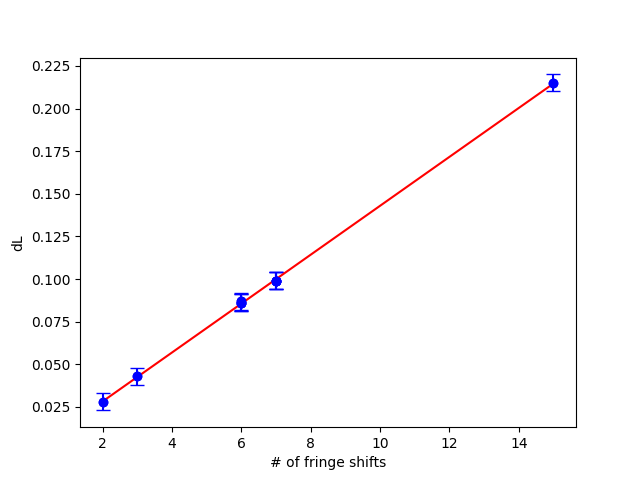
\includegraphics[scale = .5]{michelson.png}
    \caption{The number of fringe shifts counted as the variable arm is moved plotted with respect to the corresponding change in arm length. The slope of the best-fit line to this data determines the wavelength of the light being emitted when one considers an additional factor of two to account for the fact that the light has traveled down an back through the interferometer before reaching the receiver.}
    \label{fig:enter-label}
\end{figure}
To account for the fact that the light received has traveled down and back in the interferometer arms en route to the receiver, we multiply the slope of this best-fit line by two to determine the wavelength of the light, as shown in Eq. \eqref{eq:lambda}. This results in a wavelength value of 28 $\pm$ 2 mm where, again, the uncertainty calculation is shown in Appendix A. To then determine the speed of light, we use Eq. \eqref{eq:light} and multiply our determined wavelength value by the the frequency value recorded by \cite{justin}. This results in a speed of light of $3.01 \pm .021 \times 10^8$ m/s. It should be noted that this is 10$\%$ larger than the speed of light in a vacuum. Because one should expect the speed of light in air to be smaller than in a vacuum, our inferred speed of light has been corrupted by experimental imprecision. 
\section{Conclusions}
In this report, the speed of light is inferred with a Michelson interferometer. We count the number of fringe shifts that occur as a result of varying the length of one of the interferometer's arms, which allows us to determine the wavelength of light. We then use the frequency of light being generated by Pasco's transmitter, whose value is more precisely reported in \cite{justin}, and use the wave relationship to determine the speed of light in air. We find the speed of light in air to be $3.01 \pm .021 \times 10^8$ m/s, which is 10$\%$ larger than the speed of light in a vacuum. That our inferred value for the speed of light in air is greater than the accepted value for that in a vacuum is an indication of experimental error since light's speed in a vacuum will always be greater than its speed in any medium.

To make more precise inferences of the speed of light using a Michelson interferometer, the length differences of the variable arm should be programmatically measured as opposed to being approximated by eye. As an extension of this work, we recommend repeating this experimental procedure with a larger interferometer. With longer interferometer arms, the path length differences experienced by the wave of light will become more noticeable, making the peaks in the voltmeter more apparent. Although we have assumed no error in the fringe shift count, a way of programmatically determining the number of fringe shifts detected by the voltmeter should also be considered for a more accurate inference of the speed of light to ensure the assumption of zero error in the fringe shift counts. 

\appendix
\section{Uncertainty Computation}
The general formula for the uncertainty in a function with $n$ variables, $f(x^0, x^1, \dots, x^n)$, which all have uncertainties, $\delta x^0, \delta x^1, \dots, \delta x^n$ , is given as \cite{Taylor}:
\begin{equation}
    \delta f = \sqrt{\sum_{i=0}^n \left(\frac{\partial f}{\partial x^i}\delta x^i\right)^2}
\end{equation}
Since we have assumed no error in the fringe shift measurements, this results in the formula for the uncertainty in wavelength measurements:
\begin{equation}
    \delta \lambda = \frac{\partial d_L}{\partial \lambda}\delta_{d_L} = \frac{2}{\# \text{ of fringe shifts}}\delta_{d_L}
\end{equation}
Since we make multiple measurements of $\#$ of fringe shifts, the uncertainty in $\lambda$ is determined by summing over each $\#_i$ value and dividing by the total number of measurements, $N$:
\begin{equation}
    \delta_{\lambda} = \frac{\sum_{i=0}^N \delta_{d_L}2/\#_i}{N}
\end{equation}

Since we have uncertainty in the lambda measurements and \cite{justin} records uncertainties in the inferred frequency, this results in an uncertainty in the speed of light in the form:
\begin{equation}
    \delta c= \sqrt{\left(\lambda \delta_f\right)^2+ \left(f \delta_{\lambda}\right)^2}
\end{equation}
\section*{Acknowledgements}
Acknowledgments are given to Clayton Markech for support in the design of the experiment and the collection of data and to Justin wheeler for suggestions on how to operate the Pasco equipment and for providing the transmitter frequency with experimental uncertainty used in this report. 

\bibliography{sources}
\end{document}
